\chapter{機械学習 \label{c4}}
\begin{comment}
機械学習
評価指標
など
\end{comment}

\section{概要\label{c4s1}}
機械学習は,特定のタスクを効率的に処理するため,あるデータが持っているルールやパターンを反復学習を用いて学習し,そこから得られたパターンをもとに予測を行う技術である.2010年代にニューラルネットワークや自然言語処理が登場し,機械学習が再び注目されるようになった.
さらに,ハードウェアの性能の向上およびインターネットの発展により,機械学習に利用できる学習データを容易に収集できるようになったことから,ニューラルネットワークを用いた機械学習が広く用いられるようになった.ニューラルネットワークは,人体の脳の神経細胞であるニューロンおよびそのつながりである神経回路を数理モデルで表現したものである.
ニューラルネットワークが登場する前の機械学習では,データの特徴量などは人間の手によって設定されていたが,特徴量の調整などの調整は機械が自動で行うため,元のデータを与えることで,従来の人間の手による調整よりも高い精度で予測を行うことができる.

機械学習の分野の1つに自然言語処理がある.自然言語とは人間が日常的に使用している言語を指し,これをコンピュータを用いて処理する技術のことである.自然言語処理には大きく4つの段階でテキストデータの処理を行う.

\begin{enumerate}
    \item 形態素解析
    \item 構文解析
    \item 意味解析
    \item 文脈解析
\end{enumerate}

自然言語処理を行う上で,処理の対象となる文書データと,文書に含まれる単語を識別するための辞書が必要となる.自然言語処理分野において課題に挙げられることは,自然言語が本質的に持つ「曖昧さ」が挙げられ,これが文章の解釈が複雑になる要因となっている.これは,単語が持つ意味が複数存在し,その単語が用いられている文章の文脈によって意味が変化するためである.この影響を軽減させるためには,自然言語処理を行うモデルに大量のテキストデータを学習させる必要がある.

\section{二値分類における評価指標 \label{c4s2}}

\subsection{混同行列 \label{c4s2-1}}
機械学習における二値分類の評価指標に,混同行列(Confusion Matrix)がある.二値分類で出力されたクラス分類結果をまとめた行列であり,二値分類タスクを行う機械学習モデルの評価指標として利用される.
 
\begin{figure}[H]
	\centering
	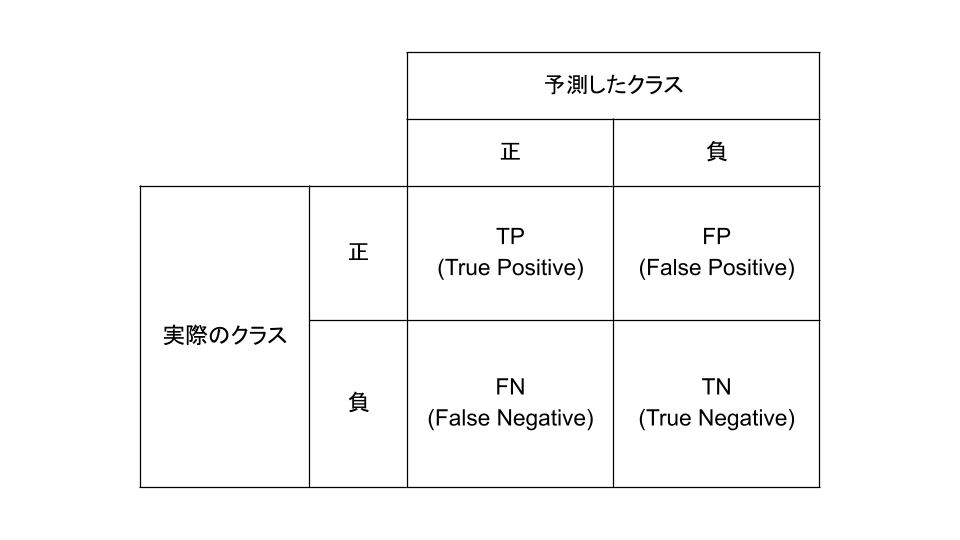
\includegraphics[width=150mm]{image/confusion-matrix.png}
	\caption{混同行列}
	\label{confusion-matrix}
\end{figure}

混同行列左上のTP(True Positive)は,実際のデータが正であるものに対し正と予想されたデータの数である.FP(False Positive)は,実際のデータが正であるものに対し負と予想されたデータである.TN(True Negative)は,実際のデータが負であるものに対し負と予想されたデータである.FN(False Negative)は,実際のデータが負であるものに対し正と予想されたデータの個数である.これら4つの値を用いて,後述する正解率,再現率,適合率,F1値を算出する.

\subsubsection{正解率 \label{c4s2-1a}}
正解率(Accuracy)は,二値分類タスクの評価指標の一つであり,全体の分類結果のうち正答した割合を示す値である.正解率の定義を次式に示す.

$$
Accuracy = \frac{TP+FN}{TP+TN+FP+FN}
$$


\subsubsection{適合率 \label{c4s2-1b}}
適合率は(Precision)は,二値分類タスクにおける評価指標の一つであり,学習モデルが正と予測したもののうち,実際に正であものの割合を示す値である.適合率の定義を次式に示す.

$$
Precision = \frac{TP}{TP+FP}
$$


\subsubsection{再現率 \label{c4s2-1c}}
再現率(Recall)は,二値分類タスクの評価指標の一つれあり,実際のデータに含まれる正クラス全体のうち,学習モデルが正と予測したものの割合を示す値である.再現率の定義を次式に示す.

$$
Recall = \frac{TP}{TP+FN}
$$

\subsubsection{F1値 (F1-score, F-measure) \label{c4s2-1d}}
F1値は,二値分類タスクの一つであり,適合率と再現率の調和平均で算出される値である.適合率と再現率の関係はトレードオフの関係であるため,適合率と再現率の間に差が生じる場合がある.この場合,精度が良いとは一概には判断できない.そのため,これら2つの調和平均を算出し,精度に対し2値のバランスを判断するために用いられる.

$$
F1 = \frac{2 \times Recall \times Precision}{Recall+Precision}
$$


\section{Attention \label{c4s3}}
Attention は,Transformer の中枢を担う仕組みである.
自然言語処理においては,単語の意味を理解するために,文中のどの単語に注目するすべきかを示すスコアである.Query:${Q}$,Key:${K}$,Value:${V}$の3つのベクトルから計算される.
${K}$と${V}$は1対1の組である.
Attentionは,Self-AttentionとSource-Target-Attentionの2種類がある.また,Attentionの算出方法は加法を使う場合と内積を使う場合があるが,Transformerで使うAttentionは内積を使って算出するため,以降のAttentionの計算は内積を使用していることを前提とする.

\subsection{Self-Attention \label{c4s3-1a}}
${Q}$, ${K}$, ${V}$は全て同じデータから得られた値を使用する.
例として「私/は/大学生/です」という文から${Q}$を得たとすると,${K}$, ${V}$も同じ文から取得する.Transformer では Encoder, Decoder の両方に採用され,文の構造や,形態素同士の関係(例文では「私」=「大学生」)を獲得するために使用される.

\subsection{Target-Attention \label{c4s3-1b}}
${Q}$,${K}$, ${V}$は異なるデータから得られた値を使用する(${K}$, ${V}$は同じデータから取得する).
例として「風邪/を/引いた」,「病院/に/行く」という2文があるとき,${Q}$は「風邪/を/引いた」から,${K}$, ${V}$は「病院/に/行く」から取得する.
 Transfomer では Decoder で採用され,「風邪/を/引いた」→「病院/に/行く」という対話の学習に用いられる.
入力文に対応する出力文が出力されるように学習を行う.

以上の Attention を基本とし,Transformers では Scaled Dot-Product Attention と Multi-Head Attentionが実装されている.
その仕組みを図aaa,図aaaに示す.

\begin{figure}[H]
	\centering
	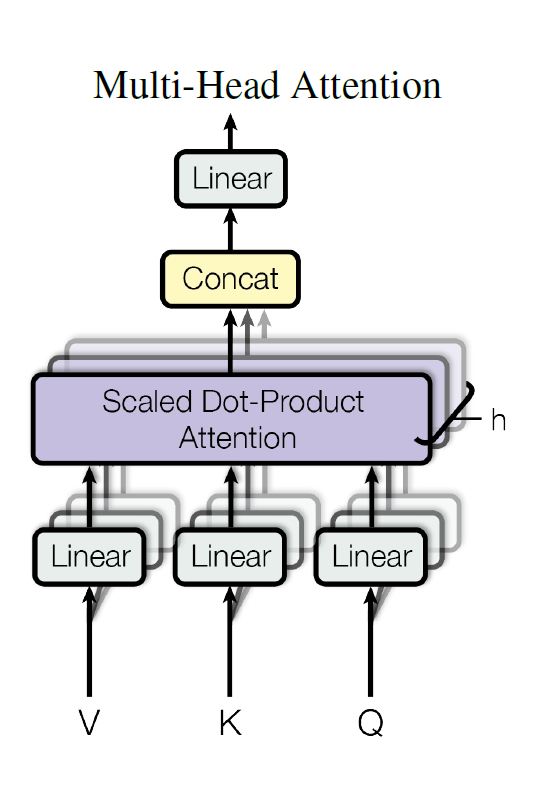
\includegraphics[width=80mm]{image/transformer-multi-head-attention.png}
	\caption{Multi-Head Attentionの構造}
	\label{mha}
\end{figure}

\begin{figure}[H]
	\centering
	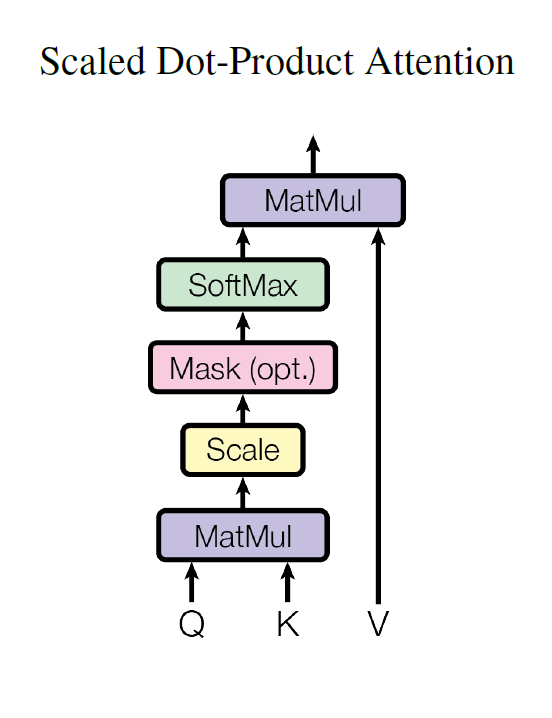
\includegraphics[width=80mm]{image/transformer-scaled-dot-product-attention.png}
	\caption{Scaled Dot-Product Attentionの構造}
	\label{sda}
\end{figure}

% 	${Q}$ ${K}$ ${V}$

\subsubsection{Scaled Dot-Product Attention}
 ${Q}$に対応する${K}$を探し,その${K}$を元にして対応する${V}$を取得する.
まず,${Q}$と${K}$の内積${QK^T}$を取ることで${Q}$に対する${K}$の関連度を算出する.
次に softmax 関数を用いて正規化する.ここで,正規化された値は,Attention の重みであり${Q}$に対応する${K}$の位置を示している.
次に Attention の重みと${V}$の内積を求め,${K}$の位置に対応する${V}$を加重和として取得する.
図 3.5 の数式を式(\ref{attention})に,softmax 関数を式(\ref{softmax})に示す.

\begin{equation}
    \mbox{Attention}(Q,K,V) = \mbox{softmax}\left( \frac{QK^T}{\sqrt{d_k}}\right)
    \label{attention}
\end{equation}

\begin{equation}
    \label{softmax}
    \frac{\exp(a_i)}{\sum_{j=1}^{n}\exp(a_j)} \quad(i=1,...,n)
\end{equation}

${QK^T}$の値は次元数に比例して大きくなり,勾配は小さくなってしまう.
そこで式\ref{attention}では${QK^T}$を${\sqrt{d_k}}$で割ることで${QK^T}$の値の増大を防いでいる.
ここで,${d_k}$は${Q}$の次元数を後述する Multi-Head Attention の Head 数で割った値である.

\begin{equation}
    \label{dk}
    d_k = \frac{Q\mbox{の次元数}}{\mbox{Multi-Head Attention のHead数}}
\end{equation}

\subsubsection{Multi-Head Attention}
Multi-Head Attention は,Scaled Dot-Product Attention を1つの Head として,複数の Head を並列で処理する仕組みである.
仮に,Head 数が 8 , ${Q}$, ${K}$, ${V}$ の次元数が 512 とすると${\frac{512}{8}=64}$であり,次元数が 64 の ${Q}$, ${K}$, ${V}$ を用いた Scaled Dot-Product Attention を並列に 8 個処理することになる.最終的には個別に計算された値を 1 つのベクトルに落とし込む(concat)ことで単語の分散表現を得る.
この Multi-Head Attention を 1 つのユニット(図 3.2 の Trm )として全結合的に接続したものが BERT モデルである.

\section{Transformer \label{c4s4}}
Transformer とは,再帰型ニューラルネットワーク (以下,RNN) を一切使わずに Attention のみを使うことで,入力と出力の文章同士の広範囲な依存関係を捉えられるモデルである.[7]
RNN は,単語が連続し順序が重要となるような時系列情報を扱うのに最適であるが,逐次的に処理を行うため,処理に多くの時間を必要とする.
また,離れた位置にある文,単語の依存関係をとらえることが難しいといった問題がある.
Transformerは以上のような問題点を克服したモデルである.
Transformerの構造を図aaaに示す.

\begin{figure}[H]%3.3
	\centering
	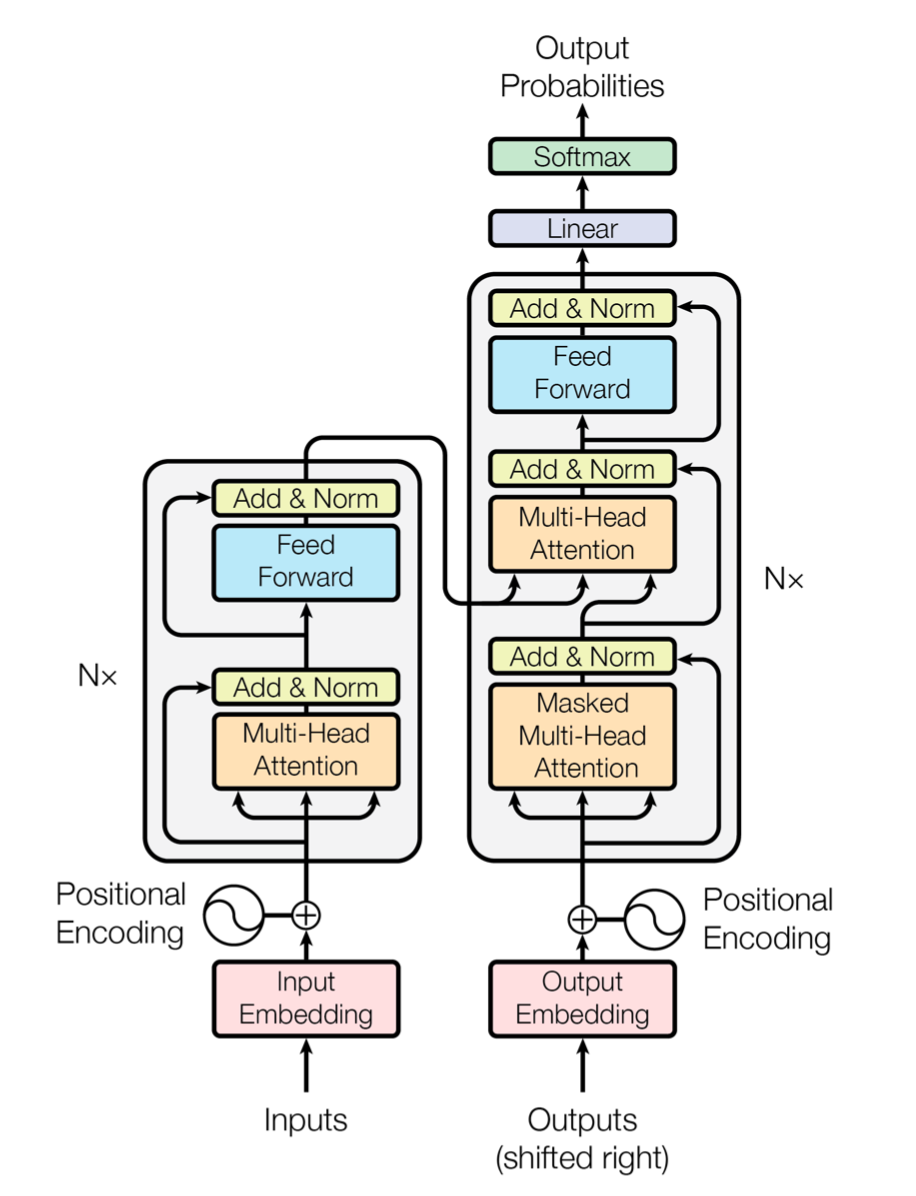
\includegraphics[width=130mm]{image/transformer.png}
	\caption{Transformerの構造}
	\label{transformer}
\end{figure}

\section{BERT \label{c4s5}}
\subsection{概要}
BERT とは,Bidirectional Encoder Representations from Transformers の略で, 「Transformerによる双方向のエンコード表現」と訳され,2018 年に Jacob Devlin らの論文[6] で発表された自然言語処理モデルである.
また,質問応答 (Question Answering) や自然言語推論 (Multi Natural Language Inference) などの 11 種の自然言語処理タスクにおいて当時の最高性能を達成している手法であり,これ以降,このモデルから派生して作られたモデルが多数存在する.また,現在のWeb検索エンジンにも用いられている.

BERT の学習は,大きく2段階に分けられる.
1つ目がラベル付けされていないデータを学習させる「事前学習」であり,2つ目が事前学習時と比較的少量のデータを用いる「Fine Tuning」である.
事前学習で汎用的なモデルを作成し,Fine Tuningを行うことで,個々のタスクに適応したモデルを作成する.

\subsubsection{事前学習}
事前学習は,大量の文章を学習することで,汎用的なモデルを形成する.
ここで得られる事前学習済みモデルをベースとして,この段階より使用するデータの量が少ない「Fine Tuning」を行うことにより,多様なタスクに対応することが可能となる.
BERTは,従来の自然言語処理モデルとは異なり,ラベルが付与されていないデータセットを利用することができる.
これにより,大量のデータを用いることが可能になる.
現状では.自然言語処理タスクのためにラベルが付与されたデータセットが少なく,入手することが困難である.
さらに,ラベルを付与する場合,そのための時間やコストがかかってしまう.
一方,インターネットが普及した現代では,ラベルが付与されていないデータは大量に存在し,容易に入手することが可能である.
そのため,BERTはデータ不足を克服した点で評価されている.
BERTの入力表現を図\ref{input}に示す.

\begin{figure}[H]
	\centering
	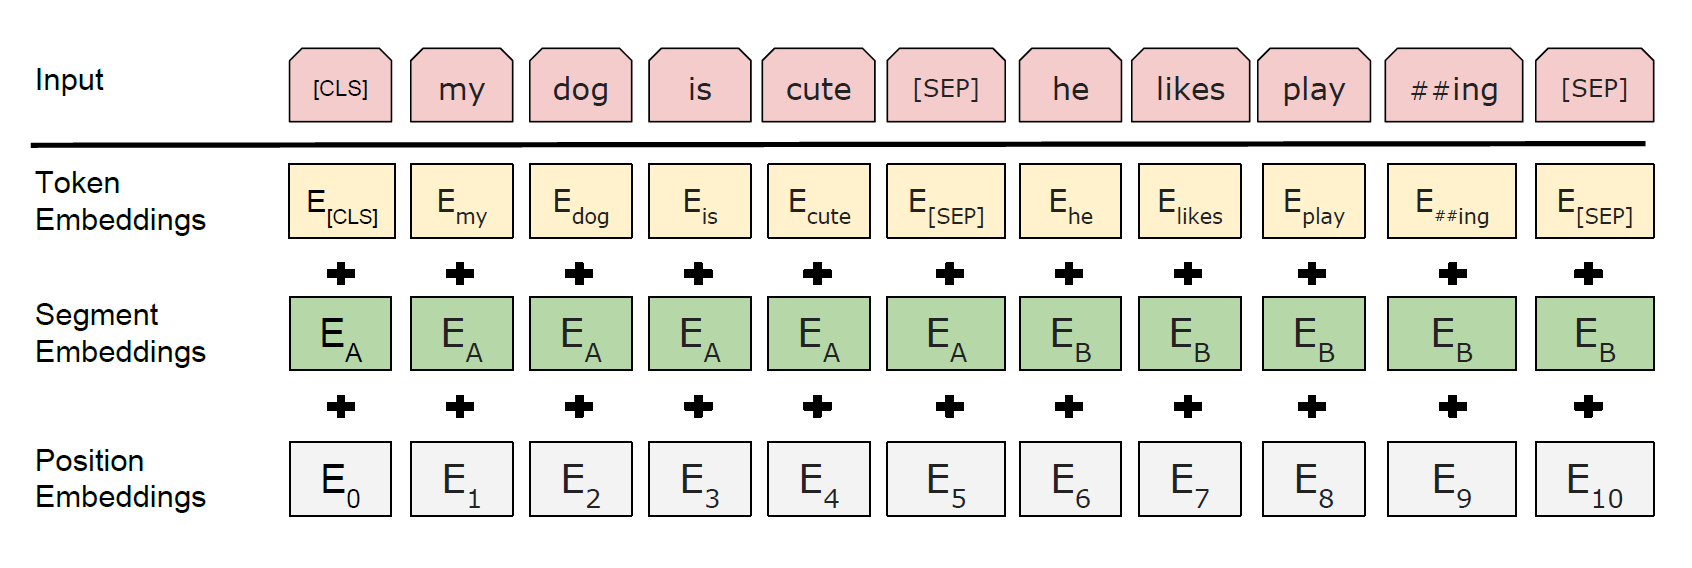
\includegraphics[width=150mm]{image/BERT-input.png}
	\caption{BERTの入力表現}
	\label{input}
\end{figure}

input では,先頭に [CLS] ,文末に [SEP] という特殊なトークンを挿入する.
[CLS] は分類タスクを解く時に使用される (それ以外のタスクではこのトークンは無視される).
[SEP] は文末であることを判別する.
また,入力文の単語数を揃えるために [PAD] トークンを挿入する場合もある.
図 3.6 の Token Embeddings は,input で入力された単語と特殊トークンをIDとして表現している.Segment Embeddings は [SEP] トークンを基準として,1 つ目の文を${E_A}$,2 つ目の文を${E_B}$のように区別した表現,Position Embedding は input 中の単語やトークンの位置を示す表現で,これらの総和が  BERT の入力表現である.

\subsubsection{Masked Language Model}
従来の自然言語処理モデルでは,文章を単一方向からでしか処理できなかった.
そのため,目的の単語より前にある文章データから予測しなければならなかった.
しかし,BERTは双方向のTransformerによって学習するため,従来の手法に比べ精度が向上した.
それを実現しているのが Masked Language Model (以下,MLM) である.入力文の 15 %の単語を確率的に別の token で置き換え,文脈から置き換える前の単語を予測させる.
具体的には,選択された 15 %のうち, 80 %は [MASK] に置き換えるマスク変換,10 %をランダムな異なる単語に変換し,残りの 10 %はそのままの単語にする.

\begin{figure}[H]
	\centering
	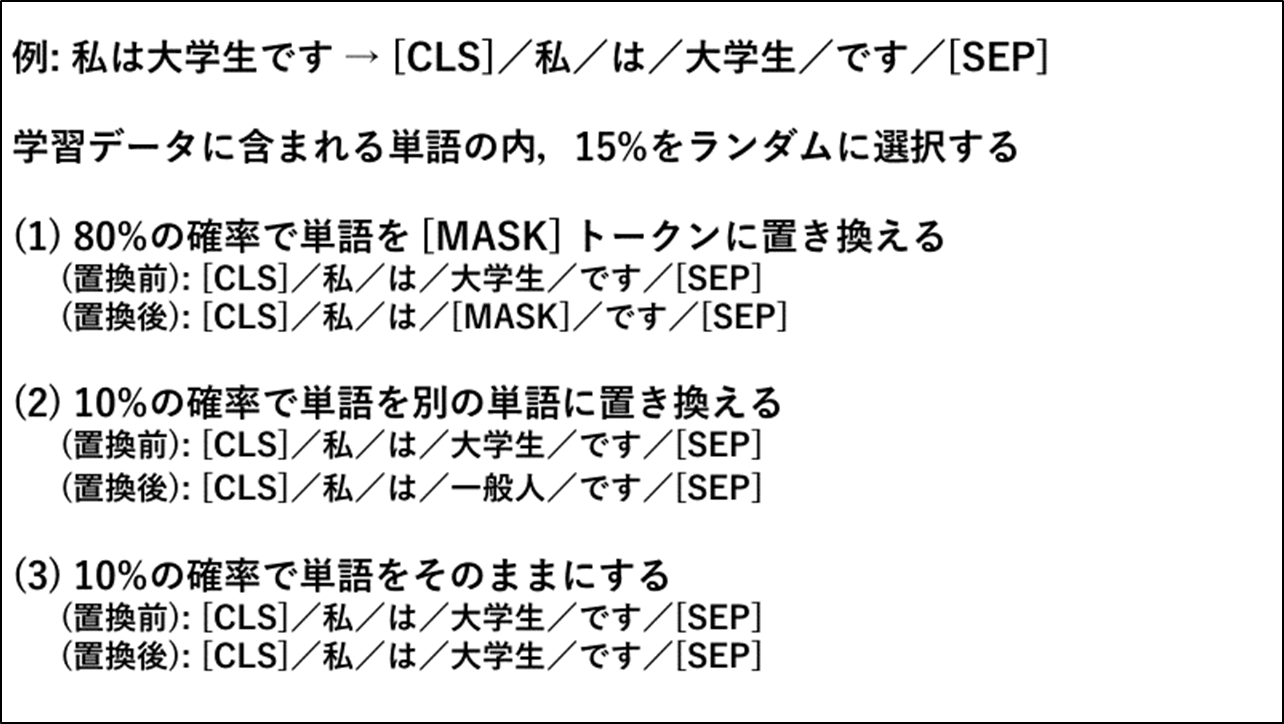
\includegraphics[width=90mm]{image/BERT-mlm.png}
	\caption{Masked Language Model の例}
	\label{mlm}
\end{figure}

\subsubsection{Next Sentence Prediction}
MLM は単語に関しての学習はできるが,文単位の学習はできない.
そこで,2 つの入力文に対して「その 2 文が隣り合っているか」を当てるよう学習する.
これにより,2 つの文の関係性を学習できる.
Next Sentence Prediction (以下,NSP) によって BERT は文章も考慮した,より広範的な自然言語処理モデルとして機能できる.
文の片方を 50 %の確率で他の文に置き換え,それらが隣り合っている(isNext)か隣り合っていない(notNext)か判別することによって学習する.
% NSPの例について画像を載せる
図\ref{nsp}のようなプロセスを大量に繰り返すことで,モデルは言語処理能力を学習する.
本研究では,穴埋め問題を解くことを前提としているため,この処理は行っていない.

\begin{figure}[H]
	\centering
	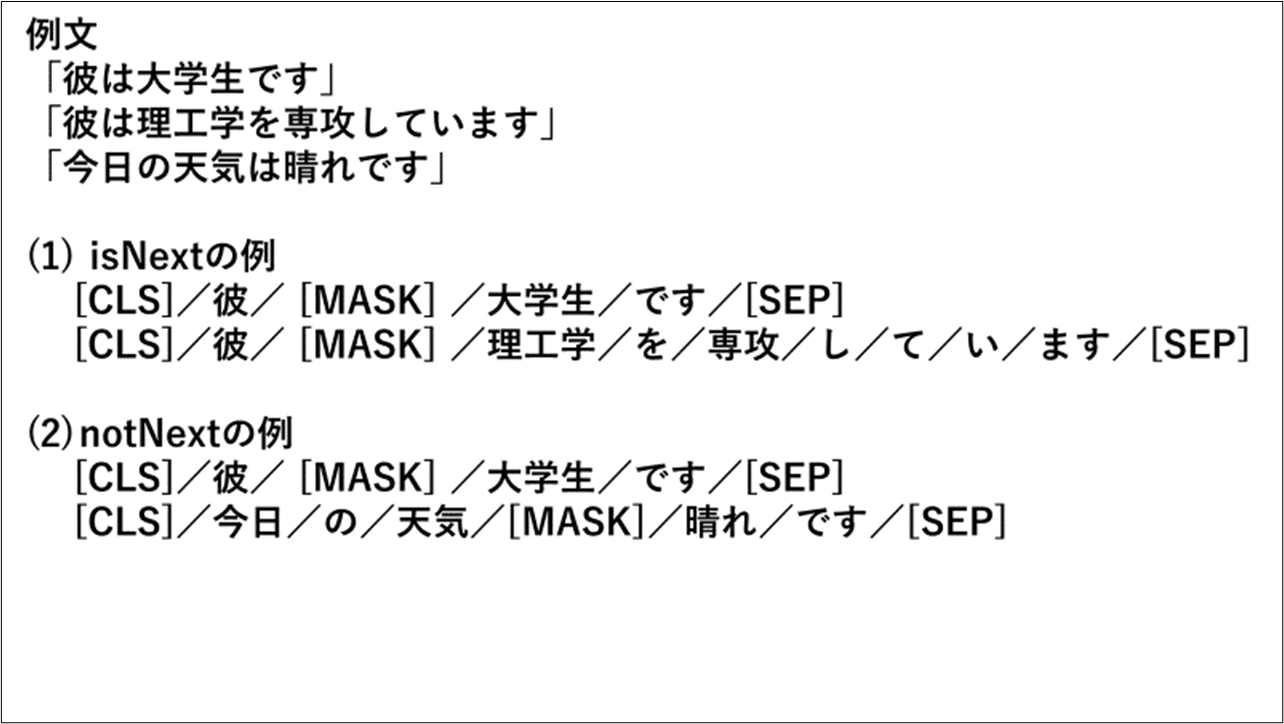
\includegraphics[width=90mm]{image/BERT-nsp.png}
	\caption{NSPの手法}
	\label{nsp}
\end{figure}

\subsubsection{Fine Tuning}
Fine Tuning とは,ある領域の知識を別の領域の学習に適用させる技術である.
従来のタスク処理モデルは特定のタスクにのみ対応している.
しかし,BERT はモデルの構造を修正せずとも,様々なタスクに応用できる.
Pretrained モデルに少量のデータでも Fine Tuning をするだけで重みを 0 から学習するのに比べて,短い時間で学習でき,過学習も抑制することができる.
BERT ではこのような汎用性の高さも評価されている.
図\ref{finetuning}に Fine Tuning の仕組みを示す.
BERT では事前学習で得られたパラメータを初期値として,図\ref{finetuning}のように各タスクごとのレイヤーを上につけて,ラベル付きデータで学習を行う.

\begin{figure}[H]
	\centering
	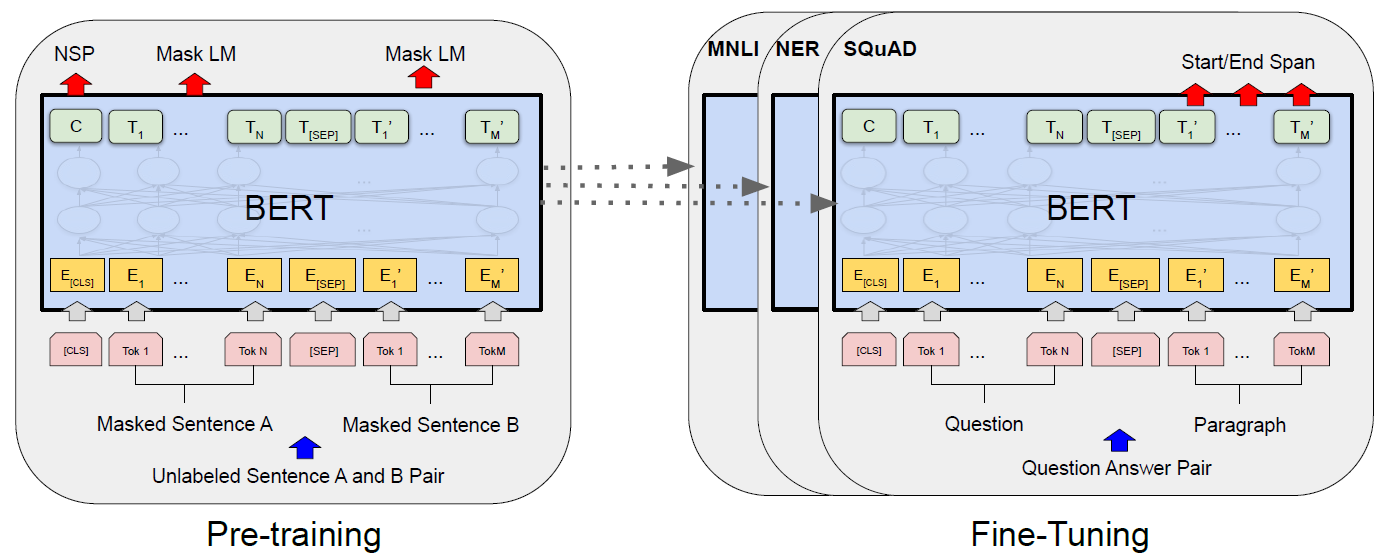
\includegraphics[width=120mm]{image/BERT-finetuning.png}
	\caption{Fine Tuning の仕組み}
	\label{finetuning}
\end{figure}



\section{LLM \label{c4s6}}
LLMとは,Large Language Model の略称であり,大規模言語モデルと呼ばれる.大規模言語モデルという用語についての正式な定義はないが,大規模コーパスを用いて事前学習を行っており,パラメータ総数が数百万以上の言語モデルを指して言われることが多い.LLMの例として,先述のBERTやOpenAI社が開発したChatGPTが挙げられる.

\subsection{ChatGPT}
ChatGPTは,2022年にOpenAI社が発表した対話型の大規模言語モデルである.ユーザが与えた指示(プロンプト)に応じた回答や情報を生成することができる.


\section{生成AI \label{c4s7}}
生成AIは,テキストや画像,音声を自律的に生成できるAI技術の総称であり,LLMは生成AIの一部とされる.
生成AIは,文章やテキスト,画像,音声などそれぞれに特化した形で作られている.文章生成であれば先述のGPT-3,GPT-3.5,GPT-4,画像生成であればStable Diffusionが挙げられる.

